\chapter{Implementierung}
\label{ch:implementation}
Die aufgestellten Anforderungen und das darauf basierende Design-Konzept kann nun in eine eigene Anwendung implementiert werden.
Dabei wird zuerst auf die Entwicklung auf iOS-Geräten eingegangen und anschließend die technische Umsetzung dokumentiert.
Bei der Umsetzung wird auf die \Gls{i18n} geachtet, sodass es im Anschluss möglich ist die Anwendung mittels \Gls{l10n} in verschiedene Sprachen zu übersetzen.\pbreak%
%
Die Nutzung der Anwendung findet idealerweise auf einem Tablet statt, da dort mehr Platz für das Zeichnen und das Vornehmen von Einstellungen bereitsteht.
Für die Entwicklung wird die Entwicklungsumgebung \textit{Xcode} verwendet, welche Gerätesimulatoren für alle zur Verfügung stehenden iOS-Geräte bereitstellt.

\section{Entwicklung auf iOS-Geräten}
\label{sec:devios}
Wenn man einen nativen Ansatz verfolgt, um eine Anwendung auf iOS-Geräten zu entwickeln, stehen einem die drei Technologien \textit{Objective-C}, \textit{Swift} und \textit{SwiftUI} zur Verfügung.
Außerdem wird die Entwicklungsumgebung Xcode, für dessen Nutzung ein macOS-Gerät notwendig ist, mit vielen hilfreichen Werkzeugen mitgeliefert.\pbreak%
%
Neben den Programmiersprachen selbst und den mitgelieferten Werkzeugen werden auch bestimmte Entwurfsmuster und Herangehensweisen empfohlen.
Die Kommunikation zwischen den bereitgestellten Schnittstellen des Herstellers und dem selbstentwickelten Programmcode ist wesentlich einfacher und verständlicher, wenn man die selbe Architektur verwendet.
Es bleibt einem trotzdem selbst überlassen, wie man das eigene Projekt aufbauen möchte.
Im Falle dieser Thesis wird sich an den empfohlenen Herangehensweisen orientiert, die auch in den folgenden Abschnitten erklärt werden.

\subsection{Objective-C und Swift}
Objective-C war lange Zeit die einzige Programmiersprache für Geräte von Apple, bis Swift im Jahre 2014 angekündigt wurde.
Des Weiteren ist Swift Open-Source und verfolgt den Ansatz plattformübergreifend genutzt werden zu können \parencite{APP2020}.
Im Vergleich zu Objective-C hat Swift eine modernere Syntax und weniger Verbosität im Programmcode.
Es wird nicht mehr in Header- und Implementierungs-Dateien unterschieden und der gesamte Aufbau erinnert an eine Kombination verschiedenster moderner Programmiersprachen.
Dies lässt sich leicht erklären, da Chris \textcite{LAT} – Hauptentwickler der Programmiersprache Swift – auf seiner Website sagte \blockquote{Of course, it also greatly benefited from the experiences hard-won by many other languages in the field, drawing ideas from Objective-C, Rust, Haskell, Ruby, Python, C\#, CLU, and far too many others to list}.\pbreak%
%
Obwohl die Programmiersprachen Swift und Objective-C beide vom selben Hersteller sind und den selben Zweck erfüllen sollen, kann man die Unterschiede beider Sprachen sehr deutlich erkennen.
Im folgenden Listing \ref{lst:objc} wird eine Beispielimplementierung einer \texttt{Vehicle}-Klasse gezeigt. Diese Klasse beinhaltet eine Methode, die zum Öffnen eines Fensters gedacht ist.
Die Methode akzeptiert genau zwei Parameter, welche beide vom Datentyp \texttt{int} sein müssen.
Als ersten Parameter muss mit \texttt{percentage} der Prozentwert der Öffnung angegeben werden und als zweiten Parameter mit \texttt{seat} übergeben werden, welches Fenster geöffnet werden soll.
Im Anschluss wird ein Objekt der Klasse erstellt und die Methode aufgerufen.
\codelisting{Implementierung der Vehicle-Klasse in Objective-C}{lst:objc}{objc-example.m}{objc}
Anders als beim Objective-C Programmcode im Listing \ref{lst:objc} zu erkennen, entfällt bei einer Swift-Implementierung im Listing \ref{lst:swift} das Einbinden von Header-Dateien komplett.
Sowohl die Deklaration als auch die Definition der Methoden und Klassen erfolgt in nur einer Datei.
Des Weiteren erkennt man, dass Methodenaufrufe und Initialisierungen von Objekten um einiges klarer und leserlicher sind, da im Vergleich zu Objective-C die umschachtelnden eckigen Klammern (\texttt{[} und \texttt{]}) entfallen.
\codelisting{Implementierung der Vehicle-Klasse in Swift}{lst:swift}{swift-example.swift}{swift}

\subsection{SwiftUI}
Seit 2019 gibt es auch die Möglichkeit mittels \textit{SwiftUI} mobile Anwendungen für Apple Geräte zu entwickeln.
SwiftUI ist dabei weniger eine eigene Sprache, sondern eher ein deklarativer Ansatz in Swift Benutzeroberflächen zu bauen.
In einfachen Swift Projekten, mit dem Ziel eine iOS-Anwendung zu entwickeln, wird für die Benutzeroberfläche das Framework \textit{UIKit} verwendet.
SwiftUI soll in Zukunft UIKit ablösen, sodass alle Anwendungen in Zukunft mittels SwiftUI entwicklet werden können.\pbreak%
%
Da SwiftUI noch relativ jung ist und regelmäßig neue Funktionen implementiert werden ist es für eine komplexere Anwendung ungeeignet.
Einfache Notizen- oder Todo-Apps lassen sich schnell und einfach bauen, doch für das Zeichnen auf Kartendaten müsste wieder auf das Framework UIKit zurückgegriffen werden.
Das hat damit zu tun, dass viele Komponenten noch nicht kompatibel für SwiftUI gemacht wurden und im Hintergrund weiterhin auf UIKit basieren.
Unter diesen Komponenten befindet sich auch die \texttt{MKMapView} aus dem \texttt{MapKit} Framework, die für das Darstellen einer Karte benötigt wird.
Es wäre theoretisch möglich die Map View innerhalb einer SwiftUI-Ansicht anzuzeigen, allerdings müsste auch hier für ein tieferes Eingreifen in die Funktionen der Map View wieder auf Swift mit UIKit zurückgegriffen werden.
Aus diesem Grund ist es sinnvoller, für die zu entwickelnde Anwendung, auf SwiftUI zu verzichten.

\subsection{Entwurfsmuster}
Es gibt viele verschiedene Möglichkeiten die Architektur einer Software aufzubauen.
Bei einfachen iOS-Anwendungen wird dafür das Entwurfsmuster \ac{mvc} verwendet.
Obwohl es möglich ist für die eigene Anwendung ein anderes Entwurfsmuster zu verwenden, lohnt es sich das bereitgestellte zu nutzen, da das \Gls{sdk} viele Werkzeuge mitbringt, die automatisiert Dateien erstellen und verwalten können, solange man sich an das \ac{mvc}-Entwurfsmuster hält.
\subsubsection{Model-View-Controller}
Das \ac{mvc}-Entwurfsmuster teilt den Programmcode in die drei Bereiche \textit{Model}, \textit{View} und \textit{Controller} auf.
Jeder dieser Bereiche hat eine eigene Zuständigkeit und sollte bis auf die Kommunikation streng von den anderen getrennt sein.
Die Einteilung ermöglicht eine bessere Wartbarkeit und Wiederverwendbarkeit von Programmcode.\\[10pt]
\begin{figure}[h!]
	\centering
	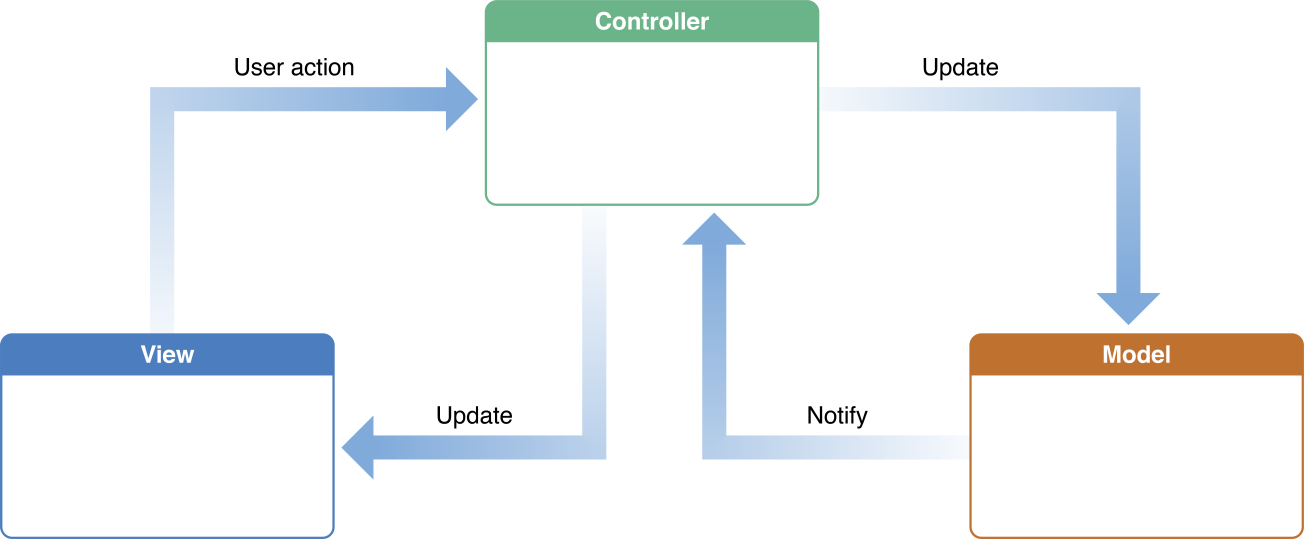
\includegraphics[scale=0.3]{images/model-view-controller}
	\caption{Darstellung der Model-View-Controller Beziehungen \parencite{APP2018}}
	\label{fig:model-view-controller}
\end{figure}
\pbreak%
Der \textbf{Model}-Bereich beinhaltet in erster Linie den Code für das Datenmodell der Anwendung, allerdings können aber auch Hilfsklassen enthalten sein, die oft verwendeten Code zusammenfassen.
Ein Model sollte nie selbst eine Referenz zu einer View oder einem Controller haben, sondern ein Controller oder eine View den Verweis zum Model.
Wie man der Abbildung \ref{fig:model-view-controller} entnehmen kann wartet das Model darauf, dass es eine Aufgabe vom Controller erhält und informiert diesen gegebenenfalls sobald die Aufgabe erfüllt wurde.\pbreak%
%
Die \textbf{View} ist der Bereich, mit dem der Benutzer interagiert.
Programmcode im View-Bereich sollte keine Geschäftslogik enthalten, sondern nur Code, welcher die View aktualisiert.
Dies könnte zum Beispiel Programmlogik zum bedingten Einfärben eines Buttons sein.
Wenn eine View Geschäftslogik benötigt, um bestimmte Aufgaben zu erfüllen, dann wird ein Verweis zu einem Model erzeugt, in dem die Geschäftslogik enthalten ist.
Auch in diesem Fall wartet die View auf Aufgaben eines Controllers, welcher zum Beispiel ein Aktualisieren der Ansicht anfordert.
Andersherum kann die View den Controller darüber informieren, dass der Benutzer eine Aktion getätigt hat, wie zum Beispiel das Drücken eines Buttons.\pbreak%
%
Die Aufgabe der \textbf{Controller} ist es zwischen den Views und den Models zu vermitteln.
Wenn es zum Beispiel Änderungen ein einem Model gibt, dessen Daten direkt an eine Ansicht gebunden sind, muss der Controller der entsprechenden View Bescheid geben die Ansicht zu aktualisieren.
Ebenso muss der Controller das Model aktualisieren, wenn der Benutzer eine Aktion auf der Benutzeroberfläche geändert hat, welche direkt mit dem Model verbunden ist.
Wie die Kommunikation zwischen den drei Komponenten funktioniert kann bei jeder Implementierung des \ac{mvc}-Entwurfsmuster unterschiedlich sein.
Bei einem iOS-Projekt wird standardmäßig das \textit{Delegation-Pattern} verwendet.

\subsubsection{Delegation-Pattern}
Das Delegation-Pattern erlaubt es bestimmte Logik über ein anderes Objekt abzubilden – also die Aufgabe zu delegieren.
Dabei kann man ein anderes Objekt einfach benachrichtigen, dass es nun etwas tun soll oder das andere Objekt etwas ``fragen`` und mit der Antwort weiterarbeiten.
In der Entwicklung von iOS-Geräten ist das Delegation-Pattern tief verwurzelt, da es in den Schnittstellen der meisten Funktionen eingebaut ist.
Möchte man innerhalb einer Anwendung auf die Ortungsdaten zugreifen, kommt man um das Delegation-Pattern nicht herum.\pbreak%
%
Um auf die Ortungsdaten zugreifen zu können würde man aus dem Framework \texttt{CoreLocation} die Klasse \texttt{CLLocationManager} nutzen.
Diesem Location Manager müsste man eine Referenz zur eigenen Klasse – beziehungsweise eine Referenz zu der Klasse, in welcher die Daten als Antowort ankommen sollen – mitgeben, die das entsprechende \Gls{protocol}, in diesem Fall \texttt{CLLocationManagerDelegate}, implementiert.
Sobald der Location Manager die Ortungsdaten des Benutzers erfasst hat nutzt er die zuvor mitgegebene Referenz zur entsprechenden Klasse und ruft dort die Funktion \texttt{locationManager(manager:didUpdateLocations:)} auf, in der die Ortungsdaten übermittelt werden.
Diese Funktion muss existieren, da dem genannten \Gls{protocol} zugestimmt wurde und es deshalb implementiert werden muss.
Fehlt die Implementierung der Funktion in der Referenz, handelt es sich dabei um einen Syntax-Fehler und das Programm kann nicht kompiliert werden.\pbreak%
%
Um die Funktionsweise des Delegation-Patterns besser darstellen zu können, wird im folgenden Beispiel der Programmcode bei einer Delegation erläutert.
Im Listing \ref{lst:engine} wird die \texttt{Vehicle}-Klasse dahingehend erweitert, dass man mit der Methode \texttt{turnKey()} den Motor starten kann (Zeile 4).
In der \texttt{Engine}-Klasse brauchen wir eine Referenz zum Fahrzeug, da der verbrauchte Kraftstoff des Fahrzeugs in der \texttt{run()}-Methode abgezogen werden muss (Zeile 17 bis 22).
Das jetzt entstandene Problem ist, dass es eine direkte Beziehung zwischen Fahrzeug und Motor gibt und die \texttt{Engine}-Klasse nicht abstrakt eingesetzt werden kann.\\
\codelisting{Implementierung der Engine-Klasse ohne Delegation}{lst:engine}{engine.swift}{swift}

Bestimmte Aufgabenbereiche kann der Motor daher an die \texttt{Vehicle}-Klasse delegieren.
Dabei muss der Motor gar nicht wissen, ob es sich dabei wirklich um die \texttt{Vehicle}-Klasse handelt oder eine andere beliebige Klasse.
Es wird als Motor nur weitergegeben, dass soeben ein Liter Kraftstoff verbraucht wurde und der Delegierte soll mit dieser Information weiterarbeiten.
Die einzige Bedingung, die von der Referenz erfüllt werden muss, ist das Implementieren des entsprechenden \Glspl{protocol}.
Dabei ist es egal welche Klasse das \Gls{protocol} implementiert.
\codelisting{Implementierung der Engine-Klasse mit Delegation}{lst:engine-del}{engine-delegation.swift}{swift}

In den Zeilen 1 bis 4 des Listings \ref{lst:engine-del} wird ein \Gls{protocol} erstellt.
Die \texttt{Vehicle}-Klasse, welches diesem \Gls{protocol} in Zeile 6 zustimmt muss die dort definierten Funktionen implementieren.
In der Zeile 10 wird dem Motor nicht mehr die Referenz zum Fahrzeug selbst übergeben, sondern zu einer beliebigen Klasse, die das \texttt{EngineDelegate}-\Gls{protocol} implementiert.
Der Motor kann absofort in den Zeilen 30 bis 35 die implementierten Funktionen aufrufen, da die Klasse sich sicher sein kann, dass die Referenz das \texttt{EngineDelegate}-\Gls{protocol} implementiert.
Im iOS-Umfeld verteilen die Controller auf diese Weise Daten zwischen den verschiedenen Ansichten.

\subsection{View Controller Lifecycle}
Für die Anzeige von Inhalten werden \textit{View Controller} verwendet.
In einer \textit{Getting Started}-Anleitung beschreibt \textcite{APP2016} den Aufbau und die Funktionsweise eines solchen Controllers, welche an dieser Stelle wiedergegeben wird.
Diese Controller bieten Grundfunktionalitäten, um Views auf dem Bildschirm anzuzeigen.
Dabei werden im Hintergrund von dem System bestimmte Funktionen aufgerufen, die sich überschreiben lassen, sodass eigene Logik hinzugefügt werden kann.
Welche Funktionen wann aufgerufen werden wird als der \textit{View Controller Lifecycle} bezeichnet.
\begin{figure}[h!]
	\centering
	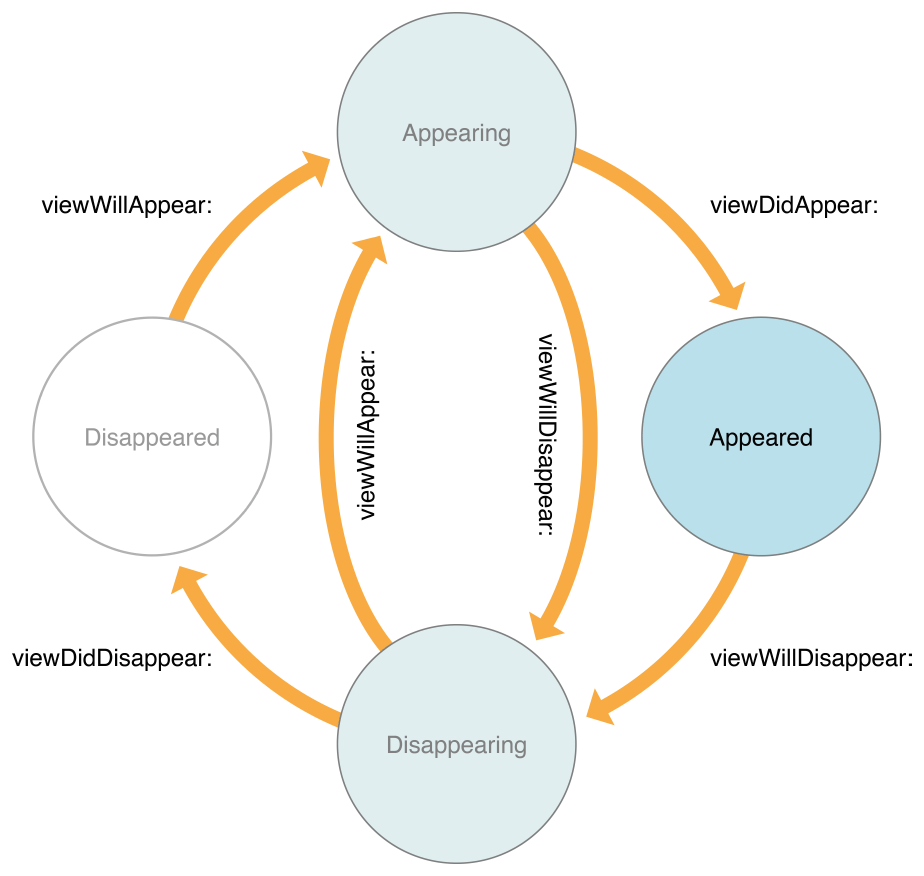
\includegraphics[scale=0.5]{images/view-controller-lifecycle}
	\caption{Darstellung des View Controller Lifecycles \parencite{APP2016}}
	\label{fig:view-controller-lifecycle}
\end{figure}
\begin{description}
\item[\texttt{viewDidLoad()}]
Wird nur einmal in einer View Controller Instanz aufgerufen.
An dieser Stelle wurde der View Controller bereits initialisiert und im Speicher abgelegt.
Benutzerdefinierter Initialisierungscode kann hier eigene Views erstellen oder Referenzen zu Models herstellen.
\item[\texttt{viewWillAppear()}]
Wird jedesmal aufgerufen, bevor die Content View des View Controllers, welche alle visuellen Komponenten enthält, angezeigt wird.
Bei Animationen zwischen den Ansichten wird diese Methode vor der Animation aufgerufen.
\item[\texttt{viewDidAppear()}]
Wird jedesmal aufgerufen, nachdem die Content View des View Controllers angezeigt wurde.
Falls eine Animation zum Anzeigen verwendet wird, kann an dieser Stelle darauf reagiert werden, wenn die Animation abgeschlossen ist.
Wichtig zu beachten ist dabei, dass die Content View nicht unbedingt sichtbar sein muss.
Es kann vorkommen, dass der Inhalt sich hinter einer anderen Ansicht befindet.
\item[\texttt{viewWillDisappear()}]
Analog zu \texttt{viewWillAppear()} wird diese Methode jedesmal aufgerufen, wenn die Content View des View Controllers von der Ansicht entfernt werden soll.
Auch hier können vorbereitende Aufgaben durchgeführt werden, wie eine Animation anzustoßen.
\item[\texttt{viewDidDisappear()}]
Analog zu \texttt{viewDidAppear()} wird diese Methode jedesmal aufgerufen, wenn die Content View des View Controllers von der Ansicht entfernt wurde.
\end{description}
Bei Aufruf der Methoden \texttt{viewWillAppear()} und \texttt{viewDidDisappear()} ist die Content View im jeden Fall nicht sichtbar, sodass es sich an diesen Stellen eignet die Benutzeroberfläche zu aktualisieren.
Findet eine Aktualisierung der Benutzeroberfläche von zum Beispiel Texten oder Listenpunkten statt, während die Content View sichtbar ist, kann der Benutzer die abrupte Änderung sehen.\pbreak%
%
Alle vorgestellten Methoden haben eine Standardimplementierung und müssen nicht überschrieben werden.
Falls eine dieser Methoden überschrieben wird, sollte die Standardimplementierung trotzdem hinzugezogen werden.
Aus diesem Grund sollte in jedem Fall am Anfang der eigenen Implementierung die Implementierung der Oberklasse ausgeführt werden.
Dies kann in der Programmiersprache Swift mit dem \texttt{super}-Keyword erreicht werden, wie im Listing \ref{lst:override} zu sehen ist.\\
\codelisting{Überschreiben einer View Controller Lifecycle Methode}{lst:override}{override.swift}{swift}

\subsection{Die Information Property List}
In jedem iOS-Projekt muss eine sogenannte \textit{Information Property List} vorhanden sein.
Diese kann als \texttt{Info.plist}-Datei an einer beliebigen Stelle im Projekt abgelegt sein, es muss nur der Pfad zu ihr hinterlegt werden.
Die Property List ist ein Key-Value-Store und basiert auf XML (siehe Listing \ref{lst:plist}).
In dieser Liste wird unter anderem der Name der Anwendung, die Version und die Buildnummer hinterlegt, sowie weitere Einstellungen vorgenommen.
Außerdem werden in der Property List auch die Begründungstexte für Berechtigungsanfragen abgelegt.
Wenn eine Anwendung versucht den Zugriff auf das Mikrofon anzufragen, allerdings kein Begründungstext hinterlegt wurde, der dem Benutzer angezeigt werden kann, wird die Berechtigung nicht angefragt.
\codelisting{Beispielinhalt einer Property List}{lst:plist}{plist-example.plist}{xml}\\
In der Information Property List können auch eigene Werte hinterlegt werden, die sowohl in der Anwendung selbst abgefragt werden können als auch in den Buildprozessen der Anwendung verwendet werden können.

\section{Technische Umsetzung}
\label{sec:techimp}
Während der Implementierung sind auch bei der technischen Umsetzung immer wieder Fragen aufgekommen.
Es gab verschiedene Möglichkeiten an bestimmte Probleme heranzugehen und diese zu lösen.
In den folgenden Abschnitten wird genauer auf diese Probleme eingegangen beziehwungsweise dargelegt, wieso sich für welchen Ansatz der teschnischen Umsetzung entschieden wurde.
\subsection{JSON Encoding und Decoding}
\label{subsec:encodingdecoding}
Alle Daten, die bearbeitet werden können, liegen im \ac{json}-Format vor.
Darunter Fallen zum Einen Indoor Architect Projektstrukturen, sowie zum Anderen die \ac{imdf}-Features, die als \ac{geojson}-Dateien abgelegt werden.
Mit Hilfe der Klasse \texttt{FileManager} kann man die Inhalte von Dateien auslesen.
Diesen Manager machen wir uns auch zu Nutze und erhalten durch Aufruf der File Manager Funktion \texttt{manager.contents(atPath: "...")} ein Objekt des Typs \texttt{Data}, wobei \texttt{"..."} eine Zeichenkette mit dem absoluten Pfad zur Datei ist.
Ein solches \texttt{Data}-Objekt enthält nun einfache Byte-Daten ohne jegliche Information, wie die Daten aufgebaut sind und in welchem Format sie vorliegen.
Für das Übertragen der Daten aus den Dateien in die Anwendung, sodass damit gearbeitet werden kann, gibt es zwei oft verwendete Möglichkeiten.
\subsubsection{Manuelles Encoden und Decoden}
Die direkte Umwandlung der Daten kann mit der \texttt{JSONSerialization}-Klasse erfolgen.
Dabei wird das \texttt{Data}-Objekt in ein \texttt{Dictionary} umgewandelt.
\codelisting{Umwandeln von JSON-\texttt{Data} in ein \texttt{Dictionary}}{lst:swift-json-decode}{swift-json-decode.swift}{swift}
In Zeile 2 des Listing \ref{lst:swift-json-decode} wird das Datenobjekt übergeben und in der Zeile 4 spezifiziert, dass das Dictionary String-Schlüssel besitzt und die Werte vom Typ \texttt{Any} sind.
Das hat damit zu tun, dass ein Wert sowohl eine einfache Zeichenkette sein kann, aber auch eine Zahl, ein Array oder ein weiteres Dictionary.
Aus diesem Grund kann kein spezieller Datentyp für die Werte angegeben werden, da sie unterschiedlich sein können.
\codelisting{Umwandeln eines \texttt{Dictionary}-Objekts in ein \texttt{Data}-Objekt}{lst:swift-json-encode}{swift-json-encode.swift}{swift}
Das Umwandeln eines existierenden Dictionaries in ein \texttt{Data}-Objekt erfolgt sehr ähnlich (Listing \ref{lst:swift-json-encode}).
Dort wird in Zeile 2 das Dictionary übergeben und man erhält das \texttt{Data}-Objekt.\pbreak%
%
Zwar ist diese Variante schnell und einfach, allerdings kann es zu einem Mehraufwand kommen, wenn man viel mit den erhaltenen Daten tut.
Da es sich bei allen Werten nun um \texttt{Any}-Typen handelt, können bestimmte Operationen nicht ausgeführt werden.
Möchte man die möglichen Werte \texttt{dict["num1"]} und \texttt{dict["num2"]} addieren, wird ein Fehler angezeigt, dass man mit zwei Werten des Typs \texttt{Any} keine Rechenoperationen ausführen kann.
Auch wenn man weiß, dass sich hinter den beiden Werten Zahlen befinden, ist es dem Compiler nicht bekannt.
Im Laufe der Anwendung müssten die entsprechenden Werte einzeln in Datentypen umgewandelt werden, die Rechenoperationen erlauben, damit man diese Werte addieren kann.\pbreak%
%
Dieser manuelle Ansatz eignet sich gut, wenn es einem unbekannt ist, in welchem Format die Daten vorliegen.
So kann man Schritt für Schritt die erhaltenen Daten analysieren und in den richtigen Datentyp konvertieren.
Da es sich in dem Fall von Indoor Architect um eine vorgeschriebene Strukur der Daten handelt ist auch zu jeder Zeit bekannt, wie das \ac{json}-Konstrukt aussieht.
Daher wurde sich dazu entschieden einen anderen Ansatz zu wählen.
\subsubsection{Encoden und Decoden mittels \texttt{Codable}}
Wenn die Struktur des \ac{json}-Objekts klar definiert ist und nicht davon abweicht, kann man mit dem \texttt{Codable}-\Gls{protocol} die Strukturen automatisch umwandeln lassen.
\codelisting{\texttt{Codable}-Struktur und dazugehörige JSON-Strukur}{lst:swift-codable-struct}{swift-codable-struct.swift}{swift}
Im Listing \ref{lst:swift-codable-struct} wird in den Zeilen 1 bis 6 eine Struktur mit dem Namen \texttt{Project} angelegt.
Damit unser automatische Ansatz funktioniert, muss diese Struktur das \texttt{Codable}-\Gls{protocol} implementieren.
Alle verwendeten Datentypen in dieser Strukur müssen ebenfalls dieses \Gls{protocol} implementiert haben.
Es können also auch eigene Datentypen erstellt und hier verwendet werden, solange sie den Anforderungen des \Glspl{protocol} gerecht werden.
In den Zeilen 8 bis 13 sieht man die in einer Datei gespeicherten \ac{json}-Struktur.
\codelisting{Automatisches dekodieren von JSON in Swift}{lst:swift-codable-decode}{swift-codable-decode.swift}{swift}
Nun kann man den \texttt{JSONDecoder} verwenden, um die Daten in eine Form zu bringen, mit der man in der Anwendung einfacher arbeiten kann (Listing \ref{lst:swift-codable-decode}).
Als Parameter für den Dekodierungsprozess kann man zum Beispiel mitgeben, dass im Snake-Case vorliegende Schlüssel (\texttt{created\_at}) zum Camel-Case (\texttt{createdAt}) konvertiert werden sollen (Zeile 2).
Außerdem kann auch spezifiziert werden, in welchem Format die Datumsfelder vorliegen (Zeile 3).
Nach dem Dekodieren lässt sich über die \texttt{project}-Variable auf die verschiedenen Daten zugreifen und entsprechende Operationen mit ihnen durchführen.
\codelisting{Automatisches enkodieren von JSON in Swift}{lst:swift-codable-encode}{swift-codable-encode.swift}{swift}
Nachdem Änderungen durchgeführt wurden können die Daten wieder enkodiert werden und in einer Datei persistent abgelegt werden.
In diesem Fall nutzt man dann analog zum \texttt{JSONDecoder} den \texttt{JSONEncoder} und spezifiziert auch hier wieder, worauf beim Enkodierungsprozess geachtet werden muss (Listing \ref{lst:swift-codable-encode}).
Nachdem die Strukur enkodiert wurde erhält man wieder ein \texttt{Data}-Objekt, welches als String in eine Datei geschrieben werden kann.\pbreak%
%
Die Verwendung dieses automatischen Ansatzes hat dafür gesorgt die Anzahl an Zeilen im Quellcode deutlich zu verringern.
Da der Aufbau der \ac{json}-Dateien immer gleich bleibt, muss nicht manuell übersetzt werden und das Enkodieren und Dekodieren der Daten zwischen Anwendung und Dateien finden in nur wenigen Zeilen statt.

\subsection{Generics}
\label{subsec:generics}
Kurz nachdem festegelgt wurde mit welchem Ansatz die Daten zwischen Dateien und Anwendung enkodiert und dekodiert werden sollen, kam es zur nächsten Schwierigkeit.
Das \acl{imdf} spezifiziert 16 verschiedene Feature-Typen, die alle unterschiedliche \ac{json}-Strukturen haben, da sie unterschiedliche Eigenschaften besitzen (siehe Listing \ref{lst:geojsonfeature} auf Seite \pageref{lst:geojsonfeature}).
Wenn nun 16 Klassen angelegt werden, damit die Struktur für jeden Feature-Typ erstellt werden kann, heißt das auch, dass 16 mal ein relativ ähnlicher Code für die Enkodierung und die Dekodierung geschrieben werden muss.
Der einzige Unterschied liegt dabei in der Kodierung der Eigenschaften.
Doch für die Kodierung der \ac{uuid}, der Geometrie und des Typs würde redundanter Programmcode in allen 16 Klassen der Feature-Typen enthalten sein.
Um dem entgegenzuwirken können \emph{Generics} verwendet werden.\pbreak%
%
Unsere globale Idee eines ``Features`` ist ein Objekt, welches immer eine \ac{uuid}, eine Geometrie, einen Typ und Eigenschaften hat.
Die Eigenschaften können dabei jedesmal unterschiedlich sein, aber die Tatsache, dass ein Feature Eigenschaften besitzt bleibt.
Da wir die Features auch kodieren wollen, fügen wir unserer Idee noch an, dass die Eigenschaften kodierbar sein müssen.
\codelisting{\texttt{Feature}-Klasse mit generischem Typ}{lst:swift-generics-feature}{swift-generics-feature.swift}{swift}
Im Listing \ref{lst:swift-generics-feature} wird nun eine Klasse definiert, welche die vier eben genannten Bedingungen eines Features erfüllt (Zeile 2 bis 5).
Da die Eigenschaften unterschiedlich sein können, wird die Klasse zu einer generischen Klasse gemacht.
Dazu wird dem Klassennamen hinzugefügt, dass ein \texttt{Properties}-Typ mit angegeben werden muss, welcher das \Gls{protocol} \texttt{Codable} implementiert (Zeile 1).
Der Name des generischen Typs (hier \texttt{Properties}) ist dabei frei wählbar.
Nun können wir der Variable, welche die Eigenschaften speichert, den generischen Typ zuweisen (Zeile 3).\pbreak%
%
Wenn eine neue Instanz der Klasse erstellt wird, können wir jetzt eine Strukur übergeben, welche den Anforderungen entspricht und die Instanz wird den generischen Typ wie den übergebenen behandeln.
Wird zum Beispiel die Struktur übergeben, die im Listing \ref{lst:swift-codable-struct} auf Seite \pageref{lst:swift-codable-struct} vorgestellt wurde, hätten wir eine gültige Feature-Instanz erstellt (Zeile 8).
Bei einer Enkodierung der Instanz würde versucht werden die Daten in eine \ac{json}-Struktur zu bringen, wie sie in den Zeilen 10 bis 20 zu sehen ist.
Um die Vorteile zu nutzen, die uns Generics bringen, können wir nun die einzelnen Klassen für die 16 verschiedenen Feature-Typen anlegen.
\codelisting{\texttt{Anchor}-Klasse, die den Anchor-Feature-Type repräsentiert}{lst:swift-generics-properties}{swift-generics-properties.swift}{swift}
Im Listing \ref{lst:swift-generics-properties} wird eine neue Klasse angelegt mit dem Namen \texttt{Anchor}, die von der \texttt{Feature}-Klasse erbt (Zeile 1).
Da es sich dabei um eine generische Klasse handelt, muss auch hier ein Typ angegeben werden, welcher für die Eigenschaften verwendet werden soll und das \texttt{Codable}-\Gls{protocol} implementiert.
Als Typ wird eine Struktur übergeben, die in der \texttt{Anchor}-Klasse selbst definiert ist und die Eigenschaften eines Anchor-Features enthält.
Wenn jetzt eine Instanz der \texttt{Anchor}-Klasse erstellt wird, muss kein Typ mehr übergeben werden, da die Klasse selbst impliziert welcher Typ verwendet werden soll.
Dazu kommt, dass die \texttt{Anchor}-Klasse von der \texttt{Feature}-Klasse erbt und deshalb auch die Enkodierung und Dekodierung anstoßen kann.
Dabei würde die Enkodierung die Daten in ein Format bringen, wie es in den Zeilen 10 bis 18 zu sehen ist.\pbreak%
%
Jetzt muss jede Klasse eines speziellen Features nur die Struktur ihrer eigenen Eigenschaften beschreiben und die Kodierung übernimmt die \texttt{Feature}-Klasse von welcher geerbt wird.

\subsection{Gesture Recognizers}
\label{subsec:gesturerecognizer}
Wie bei vielen anderen Sprachen auch werden Eingaben unter iOS mit Events abgebildet.
Eine Ansicht mit Grafiken, Texten und Bildern wird daher angezeigt und wartet auf eine Aktion, um Änderungen vorzunehmen.
Die unterschiedlichen Komponenten reagieren auch auf unterschiedliche Events.
Eine \texttt{UISwitch}-Komponente, welche einen An/Aus-Button darstellt, kann auf das \texttt{.valueChanged}-Event reagieren.
Dieses wird ausgeführt, sobald sich der An/Aus-Status des Buttons verändert.
Ein ganz normaler Button mit einem Text kann unter anderem auf die Events \texttt{.touchUpInside} oder \texttt{.touchUpOutside} hören.
Ersteres wird ausgeführt, wenn man einen Button antippt und den Button – mit dem Finger innerhalb des Buttons selbst – wieder anhebt.
Zweiteres wird ausgeführt, wenn man einen Button antippt, den Finger auf dem Bildschirm von dem Button wegbewegt und ihn im Anschluss anhebt.
Wenn man nur auf das \texttt{.touchUpInside}-Event hört, kann man dafür sorgen, dass ein Benutzer bei einem fälschlichen antippen eines Buttons noch die Möglichkeit hat die Aktion dahinter nicht auszuführen.\pbreak%
%
Für komplexere Gesten, wie das heran- und herauszoomen von Inhalten oder das rotieren von Elementen, gibt es die sogenannten \emph{Gesture Recognizer}, zu Deutsch in etwa \emph{Gesten-Erkenner}.
Diese Gesture Recognizer können jeder beliebigen Komponente angehangen werden, damit man auf die erkannten Gesten reagieren kann.
Um zu unterscheiden auf welche Gesten reagiert werden soll, kann man auf mehrere verschiedene Gesture Recognizer hören.
Die folgenden Möglichkeiten zur Gestenerkennung stehen zur Verfügung:
\begin{description}
	\item[\texttt{UITapGestureRecognizer}] Reagiert bei einem einfachen antippen. Wird in der Regel für Komponenten genutzt, die keine eingebauten Events für diesen Fall besitzen, wie zum Beispiel Bilder.
	\item[\texttt{UIPinchGestureRecognizer}] Reagiert, wenn zwei Finger sich auf dem Bildschirm bewegen und gibt Informationen zur Distanz der beiden Finger.
	\item[\texttt{UIRotationGestureRecognizer}] Reagiert, wenn zwei Finger sich auf dem Bildschirm bewegen und gibt Informationen zur Rotation der beiden Finger.
	\item[\texttt{UISwipeGestureRecognizer}] Regiert, wenn sich auf dem Bildschirm von einem Punkt A zu einem Punkt B in einer vorgeschriebenen Richtung bewegt wird.
	\item[\texttt{UIPanGestureRecognizer}] Reagiert, wenn sich auf dem Bildschirm von einem Punkt A zu einem Punkt B bewegt wird.
	\item[\texttt{UIScreenEdgePanGestureRecognizer}] Reagiert, wenn sich von einer Bildschirmkante in Richtung Mitte bewegt wird.
	\item[\texttt{UILongPressGestureRecognizer}] Reagiert, wenn ein langanhaltendes antippen stattfindet.
\end{description}
Alle aufgezählten Gesture Recognizer können unterschiedliche Parameter enthalten, die die Funktionsweise dieser bestimmt.
Anders als bei den einfachen Events, meldet sich zum Beispiel ein \texttt{UIPinchGestureRecognizer} nicht nur einmal, wenn ein ``Pinch`` stattgefunden hat.
Bei minimaler Bewegung der beiden Finger wird sich ein Gesture Recognizer immer wieder melden und darüber informieren, wie die aktuellen Parameter aussehen.
In diesem Fall wäre das die Entfernung der beiden Finger und die Geschwindigkeit, mit der sich die Distanz zwischen den Fingern erhöht oder verringert.\pbreak%
%
Für die Funktion zum Messen der Distanz zwischen zwei Orten auf der Karte wurde anfangs ein \texttt{UIPanGestureRecognizer} verwendet.
Dieser sollte beim Ausführen der Geste die Distanz zwischen dem initialen Berührungspunkt und dem Punkt, an dem die Bewegung beendet wurde, berechnen.
\codelisting{Setzen eines \texttt{UIPanGestureRecognizers} auf die Map-View}{lst:swift-gesture}{swift-gesture.swift}{swift}
Der Gesture Recognizer wurde wie im Listing \ref{lst:swift-gesture} angelegt und die minimale und maximale Anzahl von Bewegungen auf 1 gesetzt.
Dies hat zur Folge, dass der Gesture Recognizer nur reagiert, wenn nur ein Finger den Bildschirm berührt.
In der referenzierten Funktion \texttt{didPanMap} in Zeile 8 konnte dann auf die Antwort des Gesture Recognizer gewartet werden.\pbreak%
%
Dabei ist das Problem aufgetreten, dass der Gesture Recognizer als initialen Punkt nicht den Punkt zurückgegeben hat, an dem die Bewegung gestartet ist.
Es wurde der Punkt zurückgegeben, an dem der Gesture Recognizer bemerkt hat, dass eine Pan-Geste stattfindet und diese weiter verfolgt hat.
\begin{figure}[h]
	\centering
	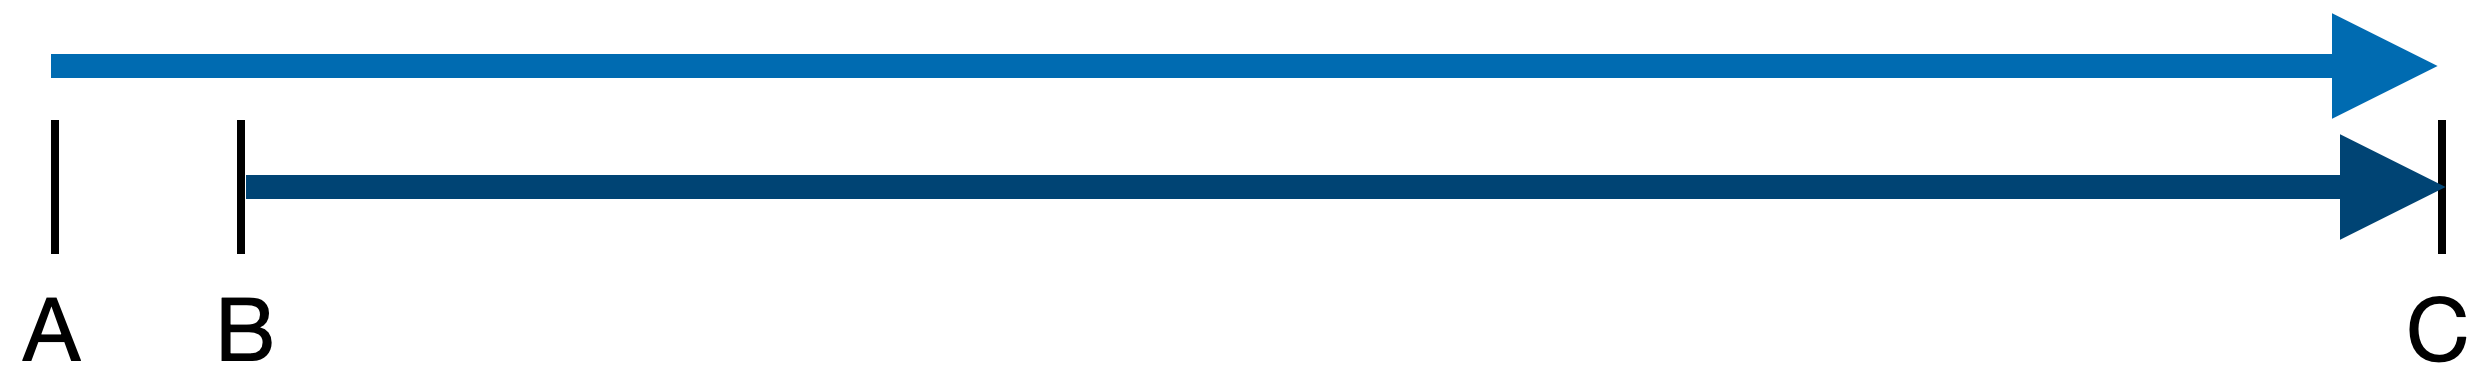
\includegraphics[scale=0.25]{images/pangesture.png}
	\caption{Visualisierung der Reaktion des \texttt{UIPanGestureRecognizer}}
	\label{fig:pangesture}
\end{figure}
In der Abbildung \ref{fig:pangesture} erkennt man, wann die eigentliche Bewegung begonnen hat (A) und wann sie beendet wurde (C).
Für den Gesture Recognizer war allerdings erst etwas später (B) klar, dass es sich gerade um eine Pan-Geste handelt.
Als Rückmeldung hat man dann den angeblichen initialen Punkt B und den Endpunkt C erhalten.
Um diesem Verhalten entgegenzuwirken musste eine eigene Implementierung des \texttt{UIPanGestureRecognizer} entwickelt werden.
\codelisting{Implementierung des \texttt{InitialPanGestureRecognizer}}{lst:swift-gesture-custom}{swift-gesture-custom.swift}{swift}
Die eigene Implementierung (zu sehen im Listing \ref{lst:swift-gesture-custom}) erbt vom \texttt{UIPanGestureRecognizer}, sodass alle internen Funktionen übernommen werden können (Zeile 4).
Zusätzlich wird eine weitere Eigenschaft angelegt, welche den echten initialen Punkt speichert, und eine Funktion zur Verfügung gestellt, die diesen Wert zurückgibt (Zeile 5 und 19).
In der \texttt{touchesBegan()}-Methode, welche aufgerufen wird sobald ein antippen bemerkt wird, kann dann der initiale Punkt gespeichert werden (Zeile 14 und 16).
Nun wird anstelle des \texttt{UIPanGestureRecognizer} der eigene \texttt{InitialPanGestureRecognizer} verwendet und es kann der echte initiale Punkt zur Berechnung der Distanz verwendet werden.

\subsection{MapKit Overlays}
Das Zeichnen von Elementen auf einer Karte in der iOS-Entwicklung ist im Grunde ganz einfach.
Es gibt eine fertige Komponenten namens \texttt{MKMapView}, welche eine leicht zu konfigurierende Kartenansicht darstellen kann.
Man kann entscheiden, ob die Position des Benutzers angezeigt werden soll oder störende Informationen, wie zum Beispiel Haltestellen und Points of Interest ausblenden.
Ebenso kann man auch einfache Elemente erstellen, wie \texttt{MKPolyline} oder \texttt{MKPolygon} und diese beliebig einfärben und konfigurieren, bevor man sie als Overlay auf die Karte legt.
Im Fall der Anwendung werden aber nicht nur fertige Elemente auf die Karte gelegt, sondern sollen auch im Entstehungsprozess visualisiert werden.
Wenn ein Benutzer ein Polygon zeichnen möchte und den Startpunkt auswählt, lässt sich aus dieser einen Koordinate kein \texttt{MKPolygon} erstellen, da für dieses Elemente mindestens drei Koordinaten vorliegen müssen.\pbreak%
%
Aus diesem Grund wurde eine Klasse erstellt, deren Aufgabe es ist die vom Benutzer ausgewählten Punkte beziehungsweise Koordinaten zu sammeln, damit daraus dann die entsprechende Visualisierung erstellt werden kann.
\codelisting{Implementierung des \texttt{MCShapeAssembler}}{lst:swift-assembler}{swift-assembler.swift}{swift}
Diese Klasse soll nur die allgemeine Aufgabe des Sammeln der Koordinaten übernehmen, während die Visualisierung von entsprechenden Unterklassen erstellt wird.
Die erstellte Klasse im Listing \ref{lst:swift-assembler}, die den Namen \texttt{MCShapeAssembler} trägt, hält eine Referenz zur eigentlichen Karte vor, auf der die Elemente gezeichnet werden (Zeile 2) und dem Overlay, welches auf der Karte angezeigt wird und das aktuell gezeichnete Element repräsentiert (Zeile 3).
Außerdem werden in der Variable \texttt{coordinates} alle gesammelten Koordinaten gespeichert (Zeile 4).
Die \texttt{add}-Funktion in den Zeilen 10 bis 12 fügt nur eine bestimmte Koordinate den gespeicherten hinzu und die \texttt{collect}-Funktion gibt die Informationen als \texttt{MKGeoJSONObject} zurück, sodass die gesammelten Koordinaten als Feature für das \acl{imdf} gespeichert werden können.
Die Funktion \texttt{renderActiveOverlay} bekommt ein Overlay übergeben, welches auf der Karte – hier referenziert über \texttt{canvas} – angezeigt wird (Zeile 18 bis 23).
Zuvor wird das aktuelle Overlay entfernt und das zu zeichnenden als neues aktives Overlay gesetzt (Zeile 19 bis 21 und 25 bis 29).
Von diesem Grundgerüst wird selbst keine Instanz erstellt, sondern die entsprechenden Unterklassen erben von dieser.\pbreak%
Als Beispiel wird im Listing \ref{lst:swift-assembler-polygon} der \texttt{MCPolygonAssembler} erklärt.
\codelisting{Implementierung des \texttt{MCPolygonAssembler}}{lst:swift-assembler-polygon}{swift-assembler-polygon.swift}{swift}
Die \texttt{add}-Funktion wird dahingehend erweitert, dass neben dem Hinzufügen der Koordinaten auch automatisch ein Overlay aus den gesammelten Koordinaten erstellt wird (Zeile 6 bis 11).
Für den Fall, dass der ``Assembler`` zwei Koordinaten kennt, wird eine \texttt{MKPolyline} als Overlay erzeugt (Zeile 8).
In Zeile 13 wird dann das soeben erstellte Overlay angezeigt, wobei das alte gelöscht und das neue gezeichnet wird.
Zur besseren Erklärung des Ablaufs einer Zeichnung kann man in Zeile 21 erkennen, wie ein solcher Assembler erstellt wird.
Sobald nun die \texttt{add}-Funktion aufgerufen wird und eine Koordinate hinzugefügt wird ist der Startpunkt bekannt und sichtbar.
Wenn man nun eine zweite Koordinate hinzufügt, wird das alte Overlay gelöscht und das neue angezeigt, welches eine Polyline ist.
Es ist also eine Linie vom Startpunkt zum Endpunkt sichtbar.
Ab der dritten Koordinate haben wir genug Daten für ein richtiges Polygon und zeigen daher auch ein Overlay als Polygon an.
\begin{figure}[h]
	\centering
	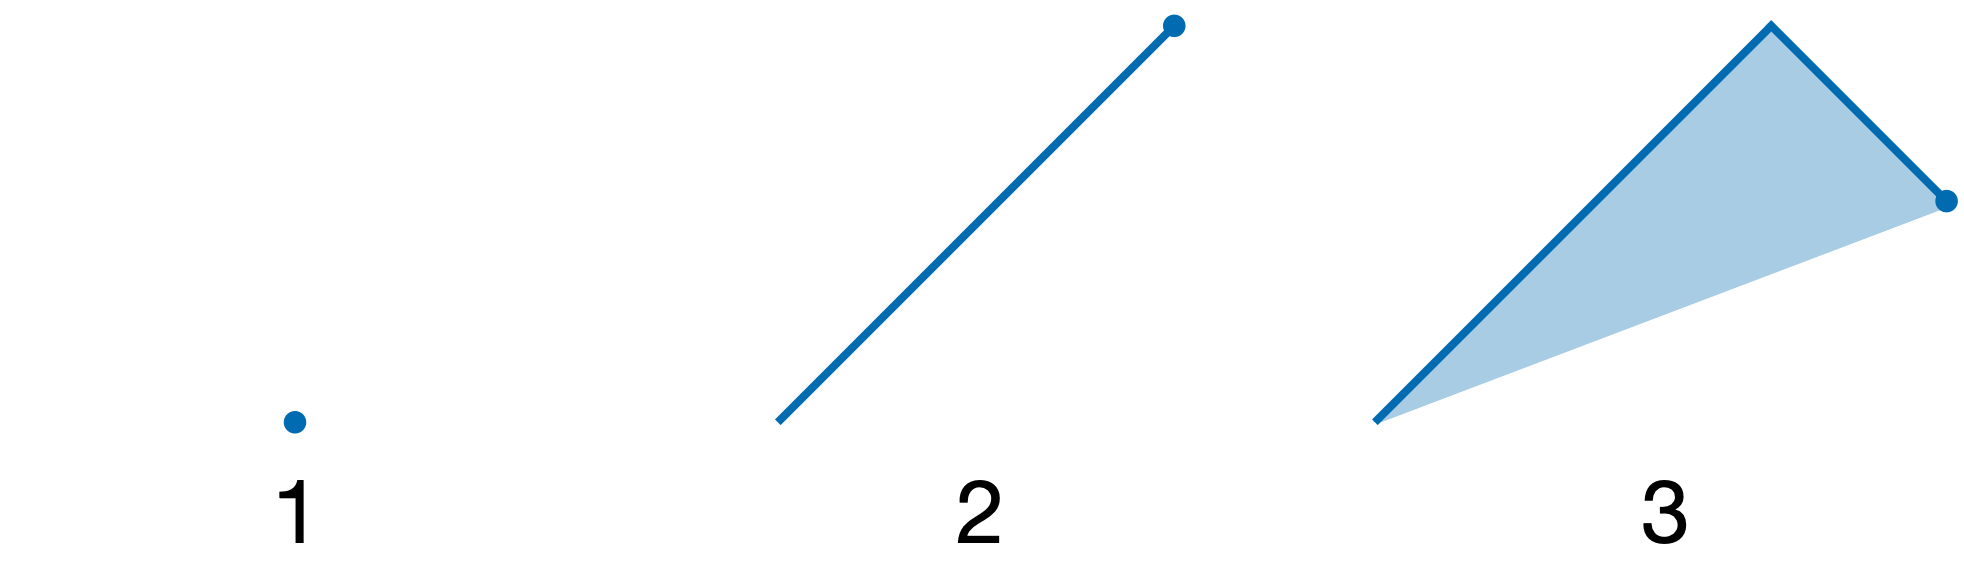
\includegraphics[scale=0.25]{images/assembler.png}
	\caption{Schritte der Visualisierung eines Polygons bei der Zeichnung}
	\label{fig:assembler}
\end{figure}
In der Abbildung \ref{fig:assembler} kann man die drei Visualisierungsschritte auf der Karte erkennen, wenn man ein Polygon zeichnet.
Bei nur einer Koordinate sieht man einen Punkt, bei zwei Koordinaten eine Linie und bei drei ein vollwertiges Polygon.

\section{Lokalisierung der Anwendung}
\label{sec:localizing}
Um Indoor Architect für eine breitere Masse an Benutzern bereitzustellen ist es wichtig, dass die Anwendung auch in den Sprachen verfügbar ist, die der Benutzer spricht.
Während des Entwicklungsprozesses musste dabei darauf geachtet werden, dass die Anwendung internationalisiert wird.
Dabei wird so entwickelt, dass im Anschluss das Übertragen der Anwendung in eine andere Sprache oder Kultur leichter gemacht wird.
Das World Wide Web Consortium (W3C) beschreibt den Prozess der Internationalisierung unter anderem als \blockquote{[d]esigning and developing in a way that removes barriers to localization or international deployment. This includes such things as enabling the use of Unicode [...]} \parencite{ISH2005}.\pbreak%
%
Bei der Internationalisierung muss neben unterschiedlichen Sprachen auch berücksichtigt werden, dass es verschiedene Schriftsysteme gibt.
Auch Grafiken sollten lokalisiert sein, da sie mögliche politische oder religiöse Sensibilitäten enthalten könnten.
Da bei Indoor Architect keine Grafiken zum Einsatz kommen, muss bei der Internationalisierung nur darauf geachtet werden, dass Texte übersetzt werden können.
Die Leserichtigung einer Sprache darf dabei nicht vergessen werden.
Mittels \emph{Autolayout} wird dafür gesorgt, dass sich die Elemente auf dem Bildschirm automatisch der Bildschirmgröße anpassen, sodass eine visuell ansehnliche Darstellung der Anwendung auf jedem Gerät erreicht wird.
Ein Teil davon ist, dass die Elemente nicht mit Begriffen wie \emph{left} und \emph{right} positioniert werden, sondern mit \emph{leading} und \emph{trailing}.
Dadurch bestimmen wir, dass zum Beispiel ein Button nicht ``link`` von einem Text ist, sondern ``vor`` dem Text.
Auf Geräten mit einer Spracheinstellung mit Leserichtung von rechts nach link bedeutet ein ``vor dem Text`` dann, dass der Button rechts neben dem Text ist.
Wenn man sich immer an diese Autolayout-Ausrichtungen hält, wird der Inhalt je nach Spracheinstellung automatisch angepasst.

\subsection{Localizable-Dictionary}
Die Übersetzung der Entwicklungssprache ist relativ einfach, wenn man sich an den Werkzeugen des \Glspl{sdk} bedient.
Wenn man eine Anwendung für eine Bibliothek entwickelt und für den Suchfilter die Kategorie ``Book`` verwenden möchte bleiben einem zwei Möglichkeiten.
\codelisting{Zuweisung eines statischen und dynamischen Strings}{lst:l10n-key}{l10n-key.swift}{swift}
In der Zeile 3 des Listings \ref{lst:l10n-key} wird ein einfacher String einer Variable zugewiesen.
Dieser Wert kann nun für den Suchfilter verwendet werden, allerdings wird in jeder Sprache der Text ``Book``angezeigt.
Anders ist es bei dem Beispiel aus der Zeile 7, in der \texttt{NSLocalizedString} verwendet wird.
Dort wird als erster Parameter der zu lokalisierende Werte in der Entwicklungssprache (die Sprache, in der die Anwendung vor der Lokalisierung entwickelt wurde) eingetragen und ein Kommentar mitgegeben.
Der Kommentar soll als Hilfe dienen, wenn man die zu lokalisierenden Texte und Grafiken exportiert und einem Übersetzer weiterleitet.\pbreak%
%
Für jede Sprache muss nun ein Unterordner im Projekt angelegt werden mit dem Format \texttt{<lang>.lproj}, wobei \texttt{<lang>} die Sprach- und Länderkennung ist.
Die Übersetzung in die deutsche Sprache hätte den Ordnernamen \texttt{de.lproj}, da die Lokalisierung auch für alle deutschsprachigen Regionen gelten soll.
In diesem Ordner muss sich eine \texttt{Localizable.strings}-Datei befinden, welche mit Key-Value-Paaren den übersetzten Text enthält, wie im Listing \ref{lst:l10n-localizable} zu sehen ist.
\codelisting{Inhalt der entsprechenden Übersetzungsdateien}{lst:l10n-localizable}{l10n-localizable.swift}{swift}
Wenn es für die ausgewählte Sprache keine Übersetzungsdatei gibt, oder kein Key-Value-Paar vorhanden ist, wird der angegebene Standardtext, in diesem Fall ``Book``, verwendet. Die Übersetzungsdatei für die englische Sprache entfällt, da es sich dabei um die Entwicklungssprache handelt.\pbreak%
%
Diese einfache Wort-zu-Wort-Übersetzung funktioniert aber nur bedingt.
Würde die Bibliothek beispielsweise Veranstaltungen anbieten, die man buchen kann, wird für die Aktion ``Buchen`` im Englischen einfach wieder ``Book`` verwendet.
Im Deutschen würde das nicht funktionieren, da das Substantiv und Verb, anders als im Englischen, unterschiedliche Wörter sind.
Aus diesem Grund wurde sich dafür entschieden in jedem Fall eindeutige Übersetzungsschlüssel zu verwenden.
\codelisting{Inhalt der entsprechenden Übersetzungsdateien (Eindeutig)}{lst:l10n-localizable-unique}{l10n-localizable-unique.swift}{swift}
Dadurch können die Texte getrennt werden und die Problematik verschwindet.
Damit auch der richtige Text im Englischen angezeigt wird, muss auch eine Übersetzungsdatei für die englische Sprache angelegt werden und eine Instanz von \texttt{NSLocalizedString} mit dem entsprechenden neuen Key erzeugt werden.\pbreak%
%
In der Abbildung \ref{fig:localized-results} kann man zwei Darstellungen der selben Ansicht sehen.
Die linke Seite nutzt die englische Lokalisierung während die rechte Seite die deutsche Lokalisierung verwendet.
\begin{figure}[h]
	\centering
	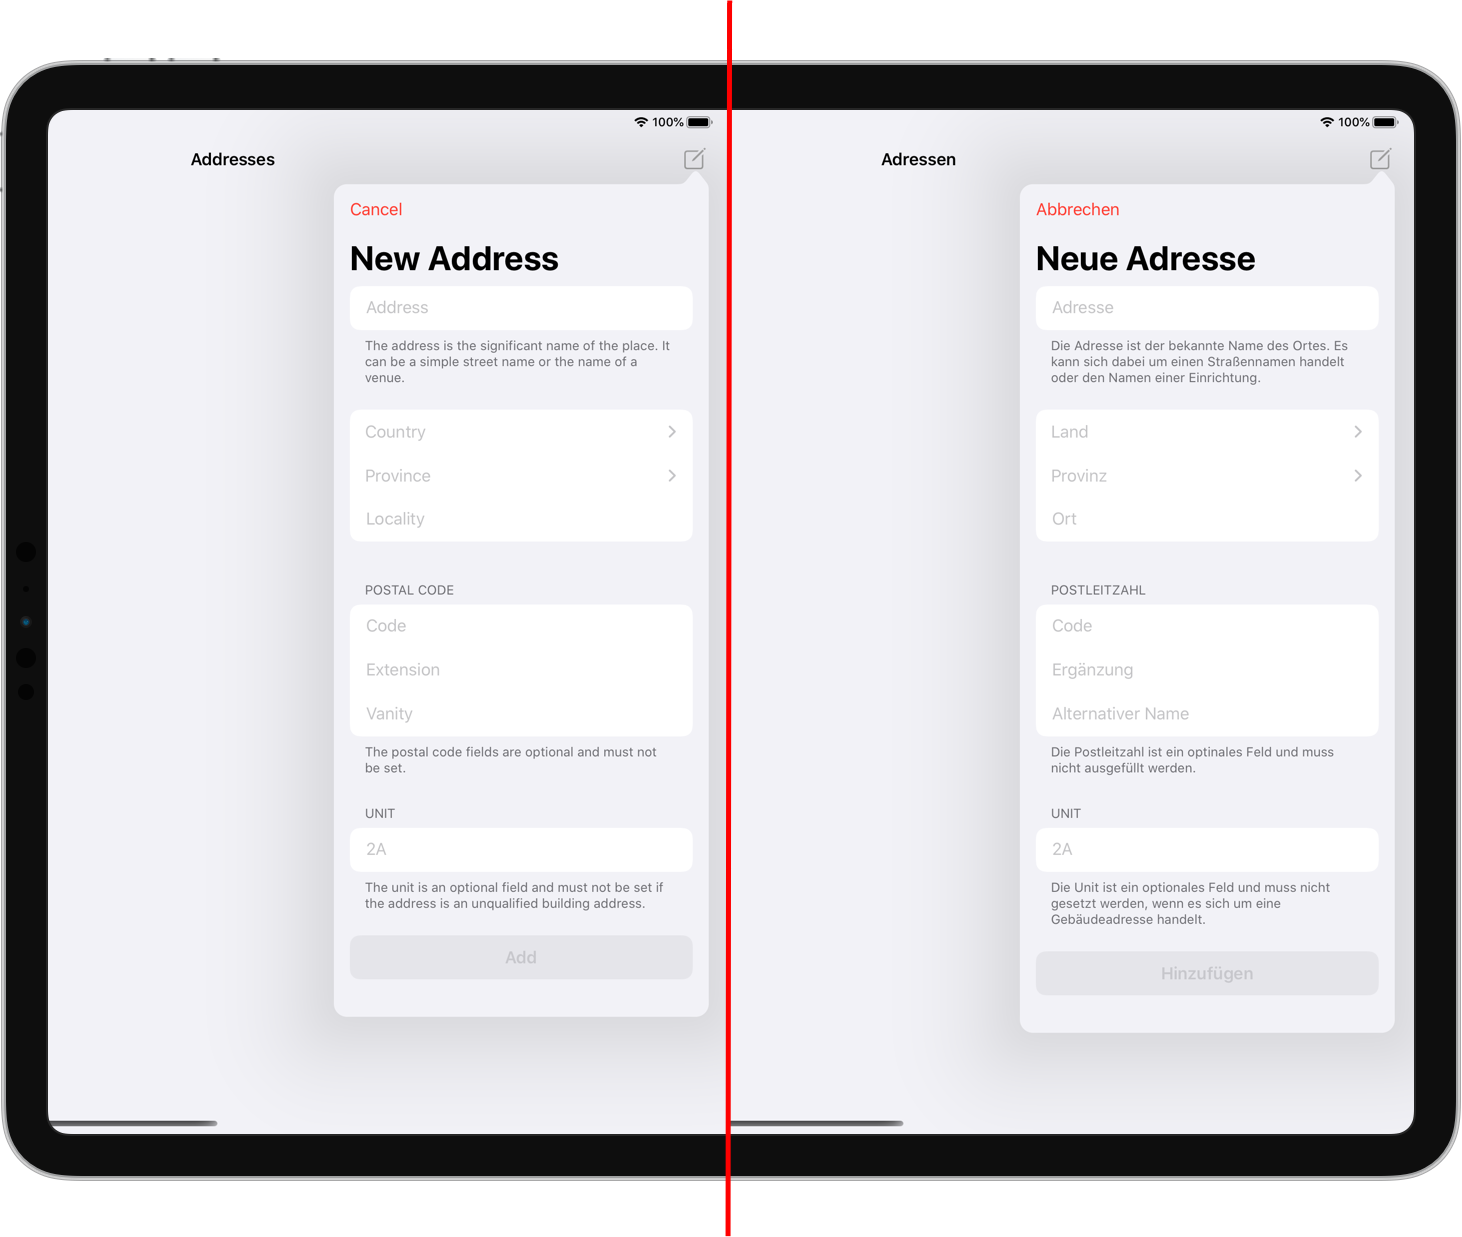
\includegraphics[scale=0.25]{images/localized.png}
	\caption{Gegenüberstellung der lokalisierten Versionen}
	\label{fig:localized-results}
\end{figure}
Viele Übersetzungen konnten vom System übernommen werden.
Der ``Cancel` beziehungsweise der ``Abbrechen``-Button wird automatisch vom System lokalisiert, sodass man für diese Fälle keine Übersetzungen anlegen muss.
Gleiches gilt für die Anzeige eines Datums oder für die Auswahl von Ländern.

\subsection{ISO Country Codes}
In dem Formular zur Erstellung einer neuen Adresse (Abbildung \ref{fig:localized-results}) muss auch ein Land ausgewählt werden.
Für diese Informationen bietet das \Gls{sdk} eine Schnittstelle an, um die lokalisierten Namen der Staaten abzufragen.
Je nach ausgewählter Sprache bekommt man zum Beispiel die Rückgabewerte \emph{Deutschland} und \emph{Österreich} oder \emph{Germany} und \emph{Austria}.
Für eine gültige \ac{imdf}-Adresse muss aber noch eine Provinz bzw. Subdivision ausgewählt werden.
Diese Informationen kann man nicht nur unlokalisiert, sondern gar nicht über die Schnittstelle abfragen.
Das Bundesland mit der ISO 3166-2 Kennung \texttt{DE-BY} würde in der deutschen Sprache \emph{Bayern} und in der englischen \emph{Bavaria} heißen.
Auf die Lokalisierung der Provinzen wurde daher verzichtet, da der Aufwand für die manuelle Lokalisierung der Provinzen aller existierenden Länder zu hoch ist.
Es wurden lediglich die Provinzen aller Länder in der entsprechenden Amtssprache manuell zusammengesucht und als Property List (Listing \ref{lst:isoprop}) abgespeichert.
Im Anschluss konnte auf die Liste der Provinzen anhand der Länderkennung zugegriffen werden.
Wurde bei der Länderauswahl das Land Belgien (\texttt{BE}) ausgewählt, wurde bei der Provinzauswahl die entsprechende Liste der Provinzen angezeigt.\clearpage
\codelisting{Ausschnitt aus der Property List mit den Provinzen der Ländern}{lst:isoprop}{isoprop.plist}{xml}
